Snap mode restricts the movement of the cursors to the points that you define. When Snap mode is on, the cursor seems to adhere, or "snap to that defined points. eCAD offers following snap modes, that you can find in Snap menu.
\begin{enumerate}
\item Free
\item Grid
\item End Points
\item Center
\item Middle Points
\end{enumerate}
\subsection{Free Snap}
By default Free Snap mode is on/checked. In free snap you have no restrictions to draw on fixed points. It allows free positioning and your drawing is not stick to the particular points but allows you drawing freely.
\begin{figure}[h!]
\centering
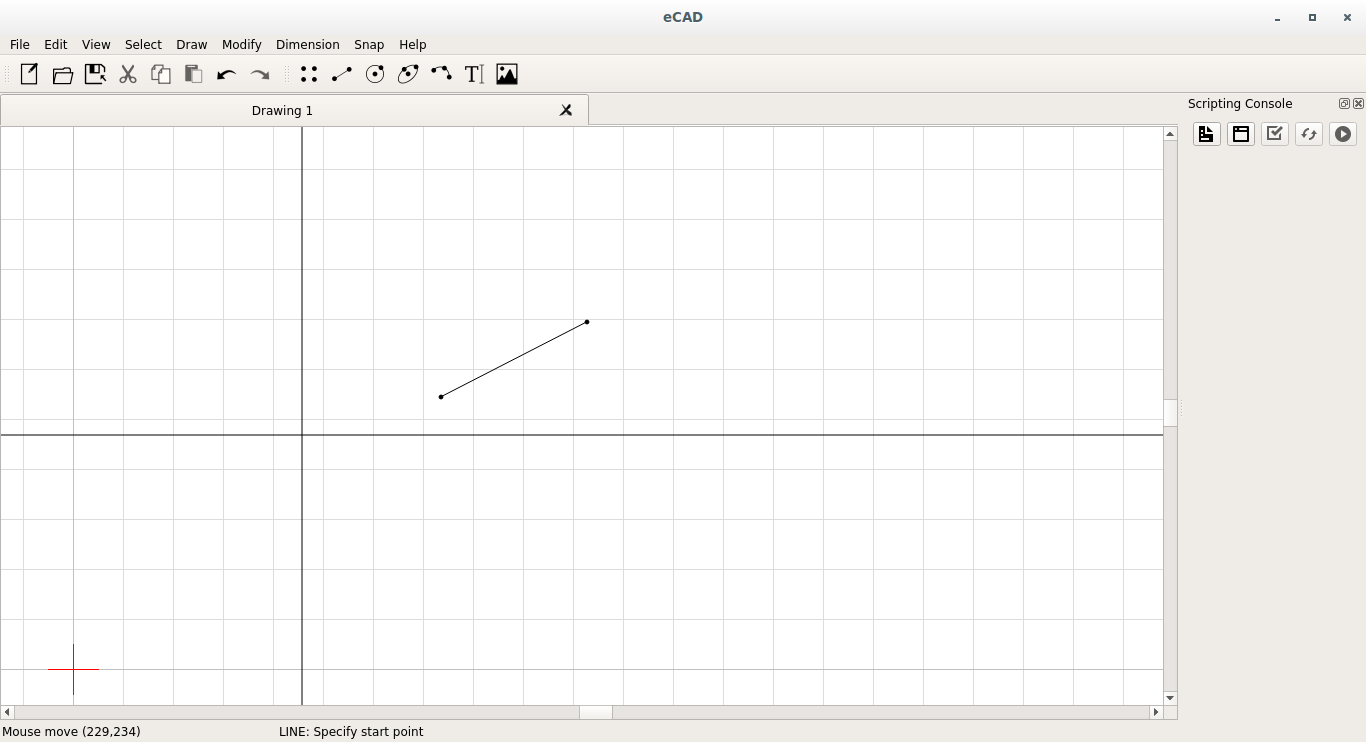
\includegraphics[width=0.8\textwidth]{images/fsnap.png}
\end{figure}
\subsection{Grid Snap}
Snaps the object(s) to the nearest grid point.
\begin{enumerate}
\item For Grid Snapping, check the Grid Snap from Snap pull-down menu.
\item Begin by drawing any entity.
\item You will notice that the grid almost seems magnetic, when you draw any object, the grid points appear to pull on it when it approaches.
\begin{figure}[h!]
\centering
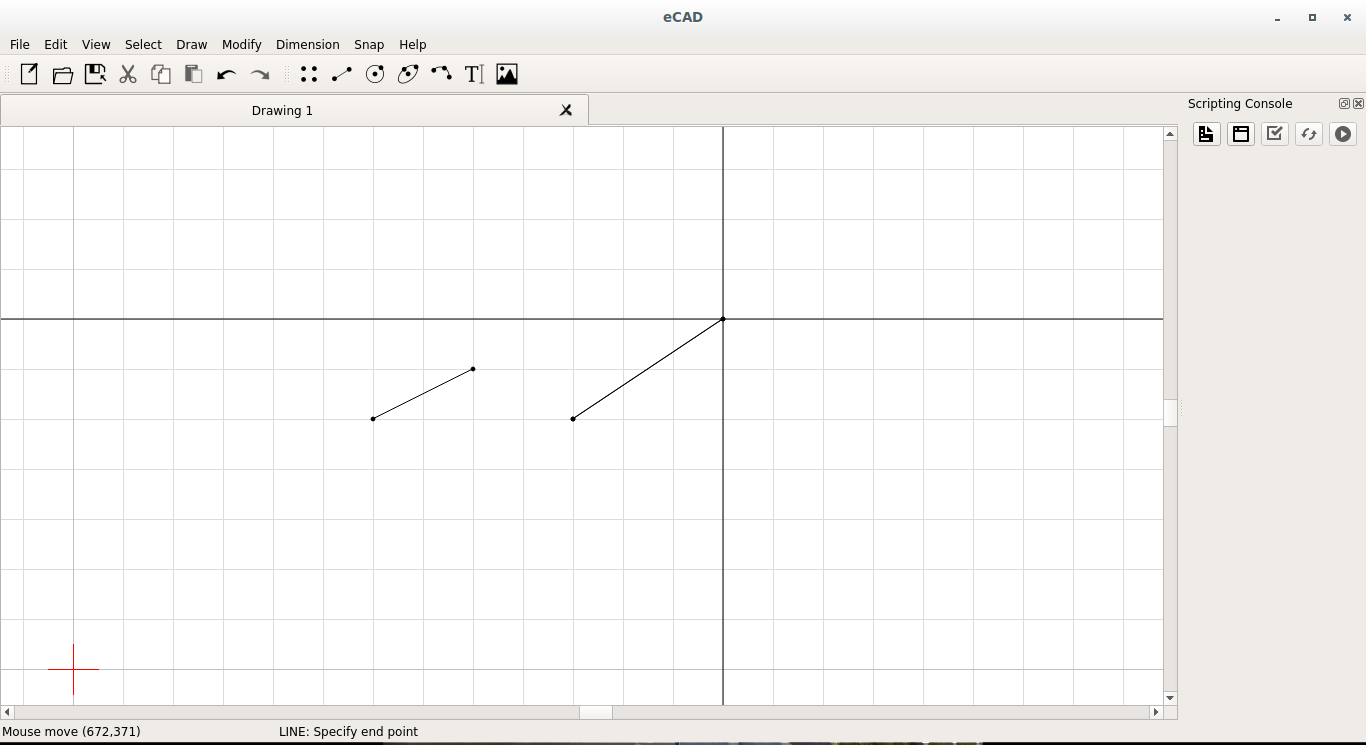
\includegraphics[width=0.8\textwidth]{images/gsnap.png}
\end{figure}
\end{enumerate}
\subsection{End Points}
This snaps used to get to the exact endpoint of a line, arc or other object that has a definite ending to it. 
\begin{enumerate}
\item Begin by drawing a line.
\item Now, Draw the second line and turn End Points mode on.
\item You will notice that the cursor automatically is pulled towards the end points.
\begin{figure}[h!]
\centering
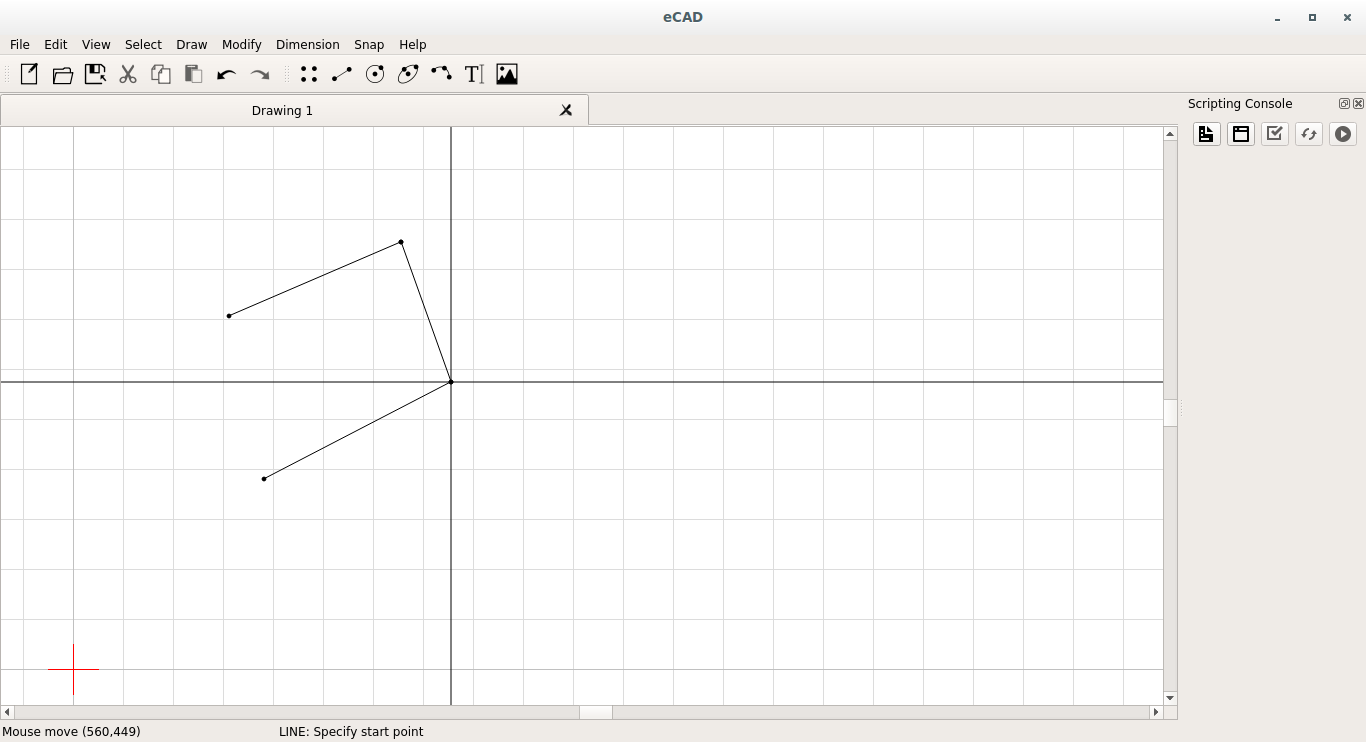
\includegraphics[width=0.8\textwidth]{images/esnap.png}
\end{figure}
\end{enumerate}
\subsection{Center}
The center snap is used to find the exact center of circles, arc and ellipses.
\begin{figure}[h!]
\centering
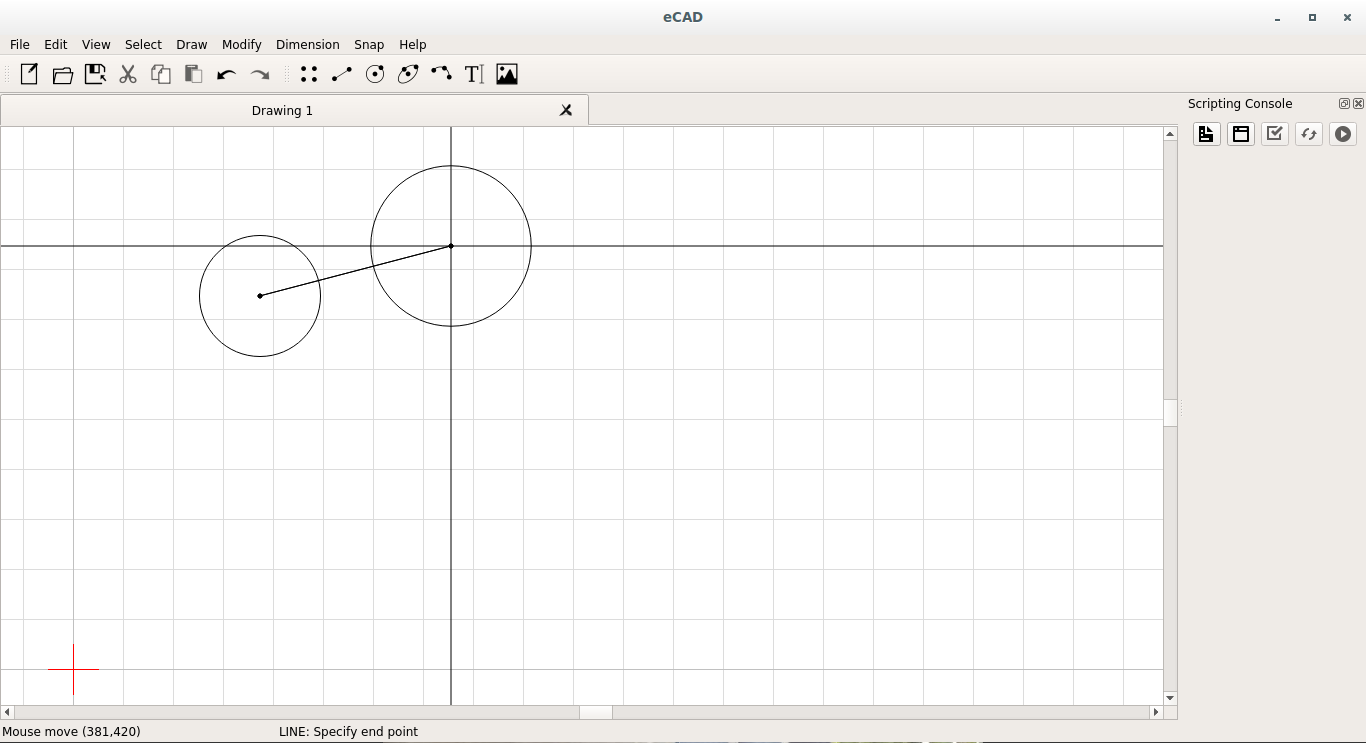
\includegraphics[width=0.8\textwidth]{images/csnap.png}
\end{figure}
\subsection{Middle Points}
This is used to find the exact middle of any object that has a beginning and an end. All lines and arcs have a midpoint. (Circle have a center, not a midpoint.)
\begin{figure}[h!]
\centering
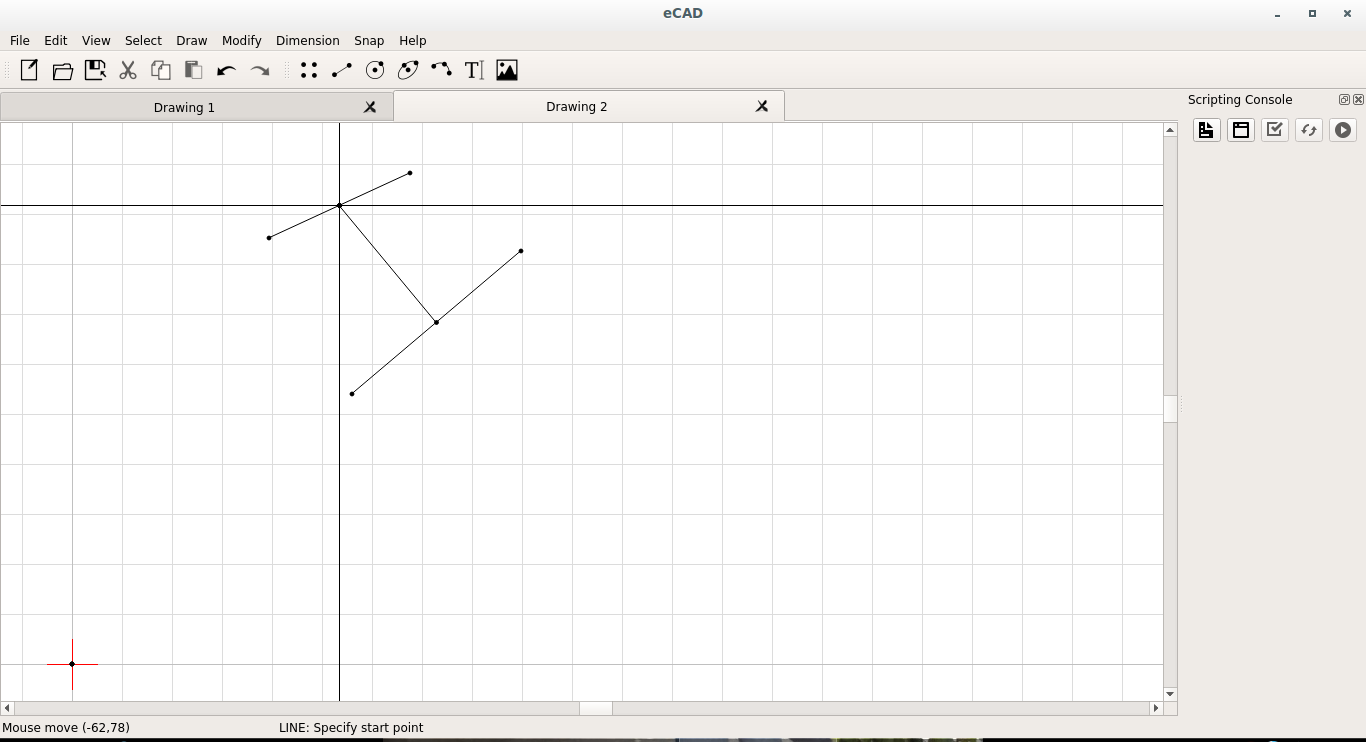
\includegraphics[width=0.8\textwidth]{images/msnap.png}
\end{figure}